\section{\textit{Teaching a Robot to Grasp}}


% ============================================================================
\subsection{Referência completa do artigo}

\begin{itemize}
  \item \textbf{Autores:} Ludovic Hamon, Philippe Lucidarme, Paul Richard, Emmanuelle Richard
  \item \textbf{Local:} LISA Laboratory, University of Angers 62, France
  \item \textbf{\textit{Journal}:} Presence: Teleoperators and Virtual Environments [Qualis B2]
  \item \textbf{Data:} June 2011
  \item \textbf{Referência:} \citeonline{bib:2011:teaching-grasp}
\end{itemize}


% ============================================================================
\subsection{Resumo}
% ..........................................................
\subsubsection{Abstract}

Humans possess the ability to perform complex manipulations without the need to consciously perceive detailed motion plans. When a large number of trials and tests are required for techniques such as learning by imitation and programming by demonstration, the virtual reality approach provides an effective method. Indeed, virtual environments can be built economically and quickly and can be automatically re-initialised. In the fields of robotics and virtual reality, this has now become commonplace. Rather than imitating human actions, our focus is to develop an intuitive and interactive method based on user demonstrations to create humanlike, autonomous behaviour for a virtual character or robot. Initially, a virtual character is built via real-time virtual simulation in which the user demonstrates the task by controlling the virtual agent. The necessary data (position, speed etc.) to accomplish the task are acquired in a Cartesian space during the demonstration session. These data are then generalised off-line by using a neural network with a back-propagation algorithm. The objective is to model a function that represents the studied task, and by so doing, to adapt the agent to deal with new cases. In this study, the virtual agent is a six-degrees-of-freedom arm manipulator, Kuka Kr6, and the task is grasp a ball thrown into its workspace. Our approach is to find the minimum number of necessary demonstrations while maintaining an adequate task efficiency. Moreover, the relationship between the number of dimensions of the estimated function and, the number of human trials is studied depending on the evolution of the learning system.

% ..........................................................
\subsubsection{Propósito do artigo}
O artigo parece tratar o problema de programar uma máquina para realizar a tarefa de rastrear um objeto, e, de acordo com sua tarefa definida, alcançar ou se afastar daquele objeto. Então acredito que seja um bom ponto de partida para a pesquisa.

% ..........................................................
\subsubsection{Técnicas utilizadas} 
\begin{itemize}
  \item Redes Neurais
  \item Programming by demonstration
  \item Virtual Reality - Simulação virtual do ambiente
  \item Cinemática Inversa
  \item Motion Capture
  \item Haptic Feedback
\end{itemize} 

% ..........................................................
\subsubsection{Contribuição em relação a artigos anteriores} %mais ou menos 10 linhas
 \begin{itemize}
   \item A forma como utiliza a percepção e planejamento simplificado do ser humano e traduz para um ponto de captura da bola através do treinamento.
   \item A forma como a rede neural é utilizada. Foi feita uma generalização no espaço cartesiano do dado registrado pela demonstração humana. A demonstração cria uma função que permite o robô se adaptar a novos casos que não haviam sido demonstrados.
   \item Estudo do impacto da variação do número de dimensões em relação ao número necessário de demonstrações. Assim é possível determinar um número mínimo de demonstrações que mantenham o nível de performance da tarefa.
 \end{itemize}  

% ============================================================================
\subsection{Metodologia}
% Descreva um pouco mais detalhadamente a metodologia e os resultados do artigo. 
% Inclua as figuras que achar mais relevantes.

\subsubsection{Motivação}
	Seres humanos têm a capacidade de realizar tarefas simples melhor do que máquinas por causa da habilidade de realizar tarefas complexas sem a necessidade de conscientemente perceber todos os detalhes do movimento. Deste modo, o movimento humano pode ser utilizado para ensinar a máquina, usando a técnica de programação por demonstração.
	O problema é realizar diversas etapas do treinamento usando máquinas reais, pois o ambiente precisa ser remontado para dar inicio a uma nova iteração. Fazendo uso de um ambiente virtual é possível realizar diversas etapas do treinamento sem necessitar de um braço mecânico real, por exemplo. O objetivo do treinamento não é que o agente imite o comportamento humano, mas que ele consiga, ao final, realizar a tarefa de maneira autônoma.
	A tarefa definida para ser realizada é  a de um braço mecânico capturar uma bola arremessada. Esse braço deve ser treinado para alcançar a bola, e segurá-la.

\subsubsection{Conceitos Utilizados}
	Captura de objetos é uma tarefa que requer soluções em tempo real, processos e modelos que representem ações humanas. Por isso a primeira tarefa é resolver a quetão da intuitividade na interação humano-robô. Assim, é possível programar rapidamente e intuitivamente. 
Artigos anteriores justificam o uso da realidade virtual como ferramenta para encurtar e diminuir os custos do processo de aprendizagem, pois pode ser construido com preço bem mais acessível e rapidamente reinicializado.
	A quantidade de testes para treinar o ator podem exceder as centenas, e por conta disso uma restauração do ambiente inicial rápida é algo tão importante.
O sistema também pode criar casos de treino a partir de captura de movimento. Um banco com movimentos é criado, e mais movimentos podem ser criados a partir da interpolação de capturas existentes, os pseudo-exemplos. 

\subsubsection{Aplicação}
	A aplicação foi escrita em C/C++ e OpenGL. A simulação contém os seguintes objetos virtuais: Uma bola, uma mão controlada pelo usuário e um braço mecânico. A bola virtual é animada de acordo com a segunda lei de newton.
	
\begin{figure}[ht]
  \centering
  
\includegraphics[height=150px]{artigos/2011-Teaching_a_Robot_to_Grasp/fig1.png}
  \caption{A simulação virtual.}
  \label{fig:2011:teaching_grasp:fig1}
\end{figure}

	O braço mecânico é chamado de Kuka Kr6. Ele possui 6 eixos de rotação. A figura \ref{fig:2011:teaching_grasp:fig2} ilustra a topologia.
\begin{figure}[ht]
  \centering
  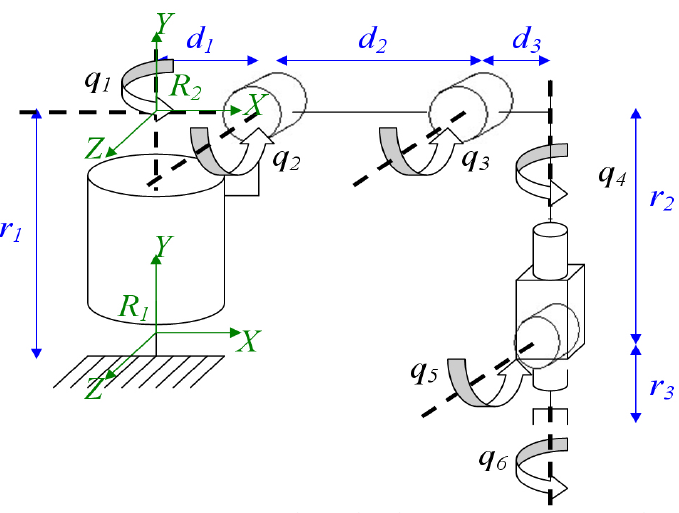
\includegraphics[height=150px]{artigos/2011-Teaching_a_Robot_to_Grasp/fig2.png}
  \caption{Parâmetros de construção do modelo de Kuka Kr6.}
  \label{fig:2011:teaching_grasp:fig2}
\end{figure}
	O agarrador tem uma posição cartesiana de acordo com os 6 ângulos dado pelo modelo geométrico direto definido por X=f(Q) onde X=(x,y,z) e Q=(q1,q2,q3,q4,q5,q6).
Para conseguir o valor dos 6 angulos de rotação, é usado a técnica geométrica inversa. Sem restrições, a área de atuação de Kuka Kr6 é definida por um torus.

\subsubsection{Interface de rastreio e captura do objeto}
	Usar um agente virtual como marionete em tempo real tem diversos problemas a respeito da área de trabalho. Como simular a restrição de movimento do braço do robô para o usuário? Uma possibilidade é o uso de interfaces hápticas.
	Isso pode ser um problema com grandes áreas de trabalho. Existem diversas técnicas para prover feedback háptico e produzir capturas de movimentos para humanos inteiros.
	Para a captura do objeto, é levantada a possibilidade do uso de luvas de RV. Porém o equipamento é frágil e ao ser usado diversas vezes para esse fim pode sofrer danos. Para contornar esse problema, outra técnica é utilizada onde uma esfera de colisão virtual é colocada no gripper do braço mecânico. A esfera tem um tamanho pre-definido e posicionada de acordo com o braço. Um mouse optico simples é utiilzado para comandar o fechamento ou abertura da mão, poupando o equipamento de captura.
\begin{figure}[ht]
  \centering
  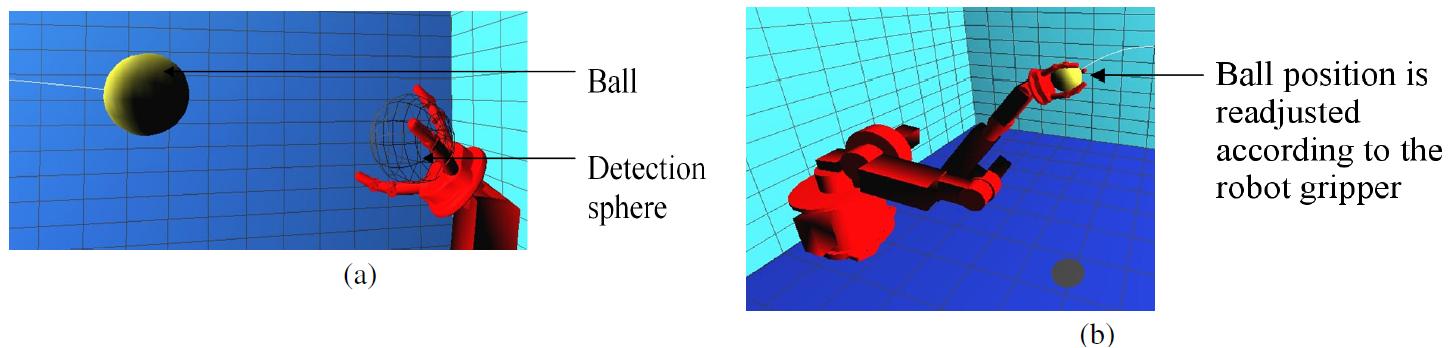
\includegraphics[width=250px]{artigos/2011-Teaching_a_Robot_to_Grasp/fig3.png}
  \caption{Sistema de grasping: (a) a esfera de colisão do grasp é renderizada apenas para visualização. (b) O centro do objeto colidiu com a esfera de colisão, e a sua posição foi reajustada para simular o grasp.}
  \label{fig:2011:teaching_grasp:fig3}
\end{figure}
	Para controlar o efetor final do robô, uma mão virtual é criada. A ideia é que a posição da mão virtual seja combinada com a posição da garra do robô. Em um dado quadro, é verificado se a mão do personagem virtual está numa posição pertencente a área de atuação do braço mecânico, e se isso acontecer, o braço é posicionado sobre a mão. O modelo geométrico inverso é utilizado para encontrar os ângulos do braço mecânico.

\subsubsection{Processo de aprendizado}
	O braço robô deve ser capaz de determinar a posição e a velocidade da bola em um determinado momento. Isso fará com que ele possa saber a trajetória da mesma, e se ela está em um espaço alcançável. Podem existir diversos pontos de encontro entre a área de atuação do braço mecâncio e a trajetória da bola.
	Para contornar o problema de definir o ponto de encontro, conhecido como “problema do encontro”, e prever a trajetória da bola, o usuário irá indicar onde o braço deve estar para agarrar a bola, toda vez que a bola é arremessada.
	Para simplificar e restringir o processo de aprendizado, algumas definições foram tomadas: A bola tem posição fixa, a trajetória é parabólica, a bola tem que passar pela área de atuação do braço mecânico. 
	Bolas são arremessadas em direção ao robô até que ele consiga agarrar 600 delas, controlado pelo humano. As bolas são jogadas com um vetor velocidade inicial aleatório.
\begin{figure}[ht]
  \centering
  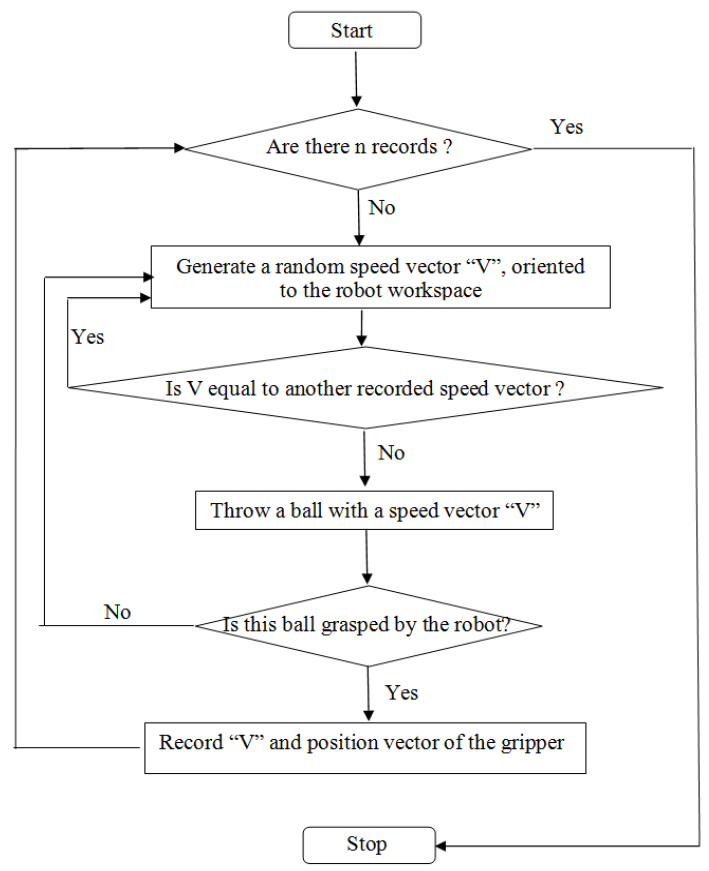
\includegraphics[height=200px]{artigos/2011-Teaching_a_Robot_to_Grasp/fig6.png}
  \caption{Diagrama do processo de demonstração. n é o número de demonstrações necessárias.}
  \label{fig:2011:teaching_grasp:fig6}
\end{figure}
	Para cada vetor de velocidade inicial, a posição da garra é registrada. O objetivo é construir uma rede neural que tenha como entrada o vetor velocidade, e como saída a posição da garra.
\begin{figure}[ht]
  \centering
  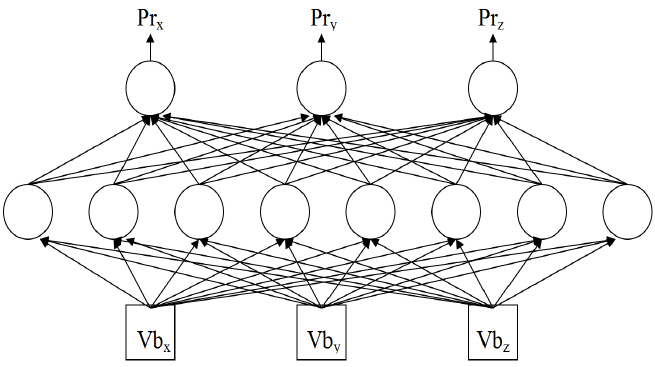
\includegraphics[height=150px]{artigos/2011-Teaching_a_Robot_to_Grasp/fig7.png}
  \caption{Diagrama da rede neural. O vetor de velocidade inicial serve de entrada, que passa por uma camada contendo 8 neurônios, e tem como saída em 3 neurônios finais as coordenadas do efetor final do braço.}
  \label{fig:2011:teaching_grasp:fig7}
\end{figure}
% ..........................................................
\subsubsection{Resultados}
A realidade virtual permitiu um aumento na eficiência da etapa de treino. Além disso, diversas medidas podem ser feitas mais facilmente a partir dos dados da simulação.

\begin{figure}[ht]
  \centering
  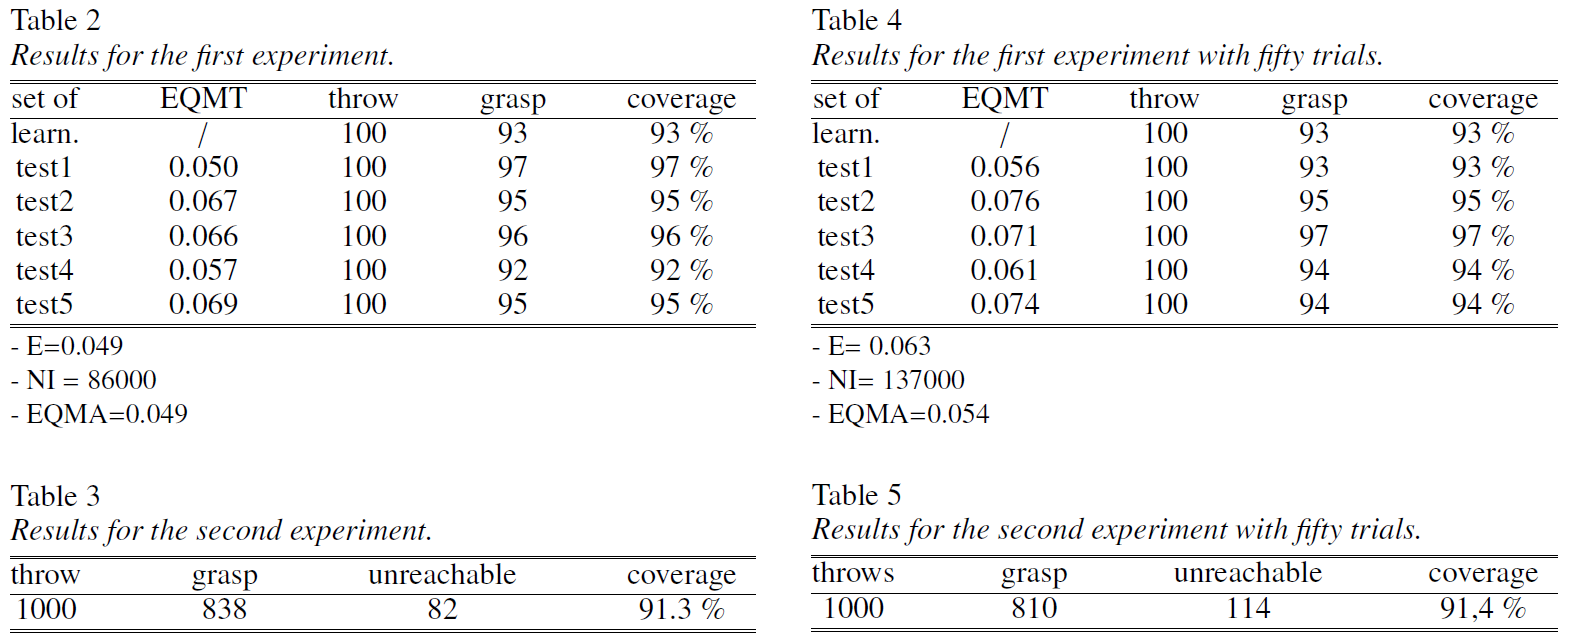
\includegraphics[width=300px]{artigos/2011-Teaching_a_Robot_to_Grasp/fig8.png}
  \caption{Tabelas contendo resultados para os experimentos.}
  \label{fig:2011:teaching_grasp:fig8}
\end{figure}

Experimento 1: Aprendizado. 100 arremessos foram realizados. A rede neural dá a posição que a garra deve atingir. O número de vezes que a garra captura a bola é contada e exibida na tabela 2. A porcentagem mostra que o agente se adaptou a novos casos, capturando mais do que durante a fase de treinamento.

Experimento 2: Eficiência. 1000 arremessos são feitos com um vetor velocidade aleatório. O numero de capturas do objeto e o numero de perdas é contado. É verificado se há vetores repetidos entre os gerados aleatoriamente. Com cobertura de mais do que 90%, o resultado é consistente com o do primeiro experimento. O agente adquiriu comportamento autônomos das demonstrações humanas com nível aceitável de eficácia.


% ============================================================================
\subsection{Pontos fortes} %no máximo três
\begin{itemize}
  \item O algoritmo proposto converge com  um numero relativamente pequeno de inputs de humanos.
  \item Demonstra um nível aceitável de eficiência.
\end{itemize}  

% ============================================================================
\subsection{Limitações} %no máximo três
\begin{itemize}
  \item Precisa da interação humana
  \item Não utiliza visão (o input da rede é um vetor velocidade). Seria preciso estimar essa velocidade com uma rede neural para dar certo.
\end{itemize} 


% ============================================================================
\subsection{Avaliação}
%\textbf{(a) Avanço considerável (\textit{Breakthrough}).}
% \textbf{(b) Contribuição significativa.}
 \textbf{(c) Contribuição modesta.}
% \textbf{(d) Contribuição fraca.}
% \textbf{(e) Sem contribuição.}
Existem outros artigos semelhantes que trazem resultados muito bons também. Foi uma boa tentativa de simplificar o processo e focar na parte da aprendizagem. Para mim, o artigo foi importante pois introduziu a ideia do uso de rede neural para treino por demonstração.

% ============================================================================
\subsection{Problema em aberto}
 \begin{itemize}
   \item Primeira extensão desse trabalho seria determinar o número mínimo de tentativas para atingir um determinado grau de eficiência. Isso requer mais estudos, mais testes e dependem das restrições e dos resultados esperados.
 \end{itemize}